\section{Which blocks of a random symplectic matrix look uniform?}

In a symplectic space a change of basis preserves alternating pairings. How many matrix entries can be observed together before those constraints become detectable? Over a fixed finite field we obtain a uniform range for all rectangular compressions. For isotropic blocks at a fixed distance from the boundary we determine the exact limiting total variation distance. The event that the matrix loses precisely one row of rank accounts for that entire distance in the limit. The input from the repository is the Fourier argument in \path{New/Spanning/SecondMoment/PositiveType.lean}, lines 102--136. There it bounds one additive character sum and is then used to estimate the mass of singular square compressions. Passing to ordered frames makes it possible to control the law of the entire matrix.

Let $V=\mathbb F_q^n$, let $G$ act on $V$ by $\pi$, and fix injections $A:\mathbb F_q^a\to V$ and $B:\mathbb F_q^b\to V^*$. For $g\in G$ let $M(g)$ be the $b\times a$ matrix whose $(i,j)$ entry is $(Be_i)(\pi(g)Ae_j)$. Take a probability mass function $\mu$ on the finite group $G$ of positive type, meaning that $(\mu(g^{-1}h))_{g,h\in G}$ is a positive semidefinite matrix. Uniform measure is one example. For $1\le j\le \min(a,b)$ write $\alpha_j$ for the maximum $\mu$-mass of the pointwise stabilizer of an independent ordered $j$-tuple in $\operatorname{im}A$, and $\beta_j$ for the analogous quantity in $\operatorname{im}B$ under the dual action. Write $R_j(a,b)$ for the number of $b\times a$ matrices of rank $j$.

\medskip\noindent\textbf{Distribution bound.}
If $g$ has law $\mu$ and $U$ is uniform on all $b\times a$ matrices, then
\[
 d_{\rm TV}(M(g),U)\le
 \frac12\left(\sum_{j=1}^{\min(a,b)} R_j(a,b)\, q^{nj}\alpha_j\beta_j\right)^{1/2}.
\]

\emph{Proof.}
A rank-$j$ matrix defining a nontrivial Fourier character factors as a sum of $j$ rank-one matrices with independent left and independent right vectors. For a fixed nontrivial additive character $\psi$ of $\mathbb F_q$, its value on $M(g)$ becomes $\psi(y(\pi(g)z))$ on $W=V^j$, for the corresponding frame $z$ and covector frame $y$ with the diagonal actions. Put $D=|W|$. In $\ell^2(W)$ take the unit Fourier vectors $c_v(w)=D^{-1/2}\psi(-v(w))$ and the point masses $e_w$. Choose vectors $u_g$ with Gram matrix $\mu(g^{-1}h)$, with inner product conjugate-linear in the first argument. The inner product of
\[
 \sum_{g\in G} c_{g y}\otimes u_g
       \quad\hbox{and}\quad
 \sum_{h\in G} e_{h z}\otimes u_h
\]
is $|G|D^{-1/2}\sum_t\mu(t)\psi(y(\pi(t)z))$.
Their squared norms are $|G|\mu(\operatorname{Stab}y)$ and $|G|\mu(\operatorname{Stab}z)$ by orthonormality. Cauchy--Schwarz therefore bounds the squared modulus of the Fourier coefficient by $D\alpha_j\beta_j$. The $\ell^1$--$\ell^2$ inequality and Parseval give the displayed estimate, since the uniform distribution has zero Fourier coefficient at every nontrivial character.\hfill$\square$

\medskip\noindent\textbf{Symplectic compression theorem.}
For even $n$, $g$ uniform in $\operatorname{Sp}_n(\mathbb F_q)$, and arbitrary $A,B$ as above with $a+b\le n$, an absolute constant $C$ gives
\[
 d_{\rm TV}(M(g),U)\le C q^{-(n+1-a-b)/2}.
\]
Thus $n-a-b\to\infty$ suffices at fixed $q$, uniformly in both subspaces. For every fixed integer $c\ge0$, the dimensions $n=2m$, $a=m$, $b=m-c$ admit isotropic choices such that the distance stays bounded away from zero as $m\to\infty$.

\emph{Proof of the upper bound.}
The symplectic form identifies the dual action with the given one. By Witt extension, the orbit of an independent $j$-frame consists of all independent frames with its prescribed alternating Gram matrix. Once $i-1$ independent vectors have been specified, the pairings with the next vector give $i-1$ independent linear constraints. Of the $q^{n-i+1}$ solutions at most $q^{i-1}$ are in the previous span. Since $j\le n/2$, every orbit has size at least
\[
 q^{nj-j(j-1)/2}\prod_{i=1}^j(1-q^{2i-2-n})
 \ \ge\ q^{nj-j(j-1)/2}\prod_{k\ge1}(1-2^{-2k}).
\]
Each stabilizer mass is the reciprocal of its orbit size. Factoring rank-$j$ matrices through $\mathbb F_q^j$ and dividing by $|\operatorname{GL}_j(\mathbb F_q)|$ gives
$R_j(a,b)\le q^{j(a+b-j)}/\prod_{k\ge1}(1-2^{-k})$.
Substitution leaves a geometric sum $\sum_{j\ge1}q^{-j(n+1-a-b)}$, as claimed.\hfill$\square$

\emph{Proof of the obstruction.}
Under the symplectic identification take $\operatorname{im}A$ Lagrangian and $\operatorname{im}B=W_0$ isotropic of dimension $m-c$. Then $L=g\operatorname{im}A$ is a uniform Lagrangian. Full row rank of $M(g)$ means $L\cap W_0=0$, since $L^\perp=L$. The number of Lagrangians in dimension $2m$ is $\prod_{k=1}^m(q^k+1)$, as follows by counting pairs of a Lagrangian and a line in it and passing to the line's symplectic quotient. A fixed $i$-dimensional subspace of $W_0$ lies in $L$ with probability $1/\prod_{k=m-i+1}^{m}(q^k+1)$, by the same quotient argument. Subspace-lattice M\"obius inversion gives the full-rank probability
\[
 P_{m,c}=\sum_{i=0}^{m-c}
  \frac{(-1)^i q^{i(i-1)/2}\genfrac{[}{]}{0pt}{}{m-c}{i}_{q}}
       {\prod_{k=m-i+1}^{m}(1+q^k)},
\]
where the Gaussian coefficient counts $i$-subspaces of $W_0$ and the M\"obius function in dimension $i$ is $(-1)^i q^{i(i-1)/2}$. For $c=0$ the probability also has the elementary form $\prod_{k=1}^m(1+q^{-k})^{-1}$, since there are $q^{m(m+1)/2}$ Lagrangian complements, parametrized by symmetric matrices.

Set $Q=q^{-1}$. The $i$th term converges to $(-Q^{c+1})^i/\prod_{k=1}^i(1-Q^k)$ and is bounded in absolute value by $Q^{(c+1)i}/\prod_{k\ge1}(1-Q^k)$. These facts follow by extracting the highest powers of $q$ in the Gaussian coefficient and the denominator. Dominated convergence and the power-series identity
$\sum_{i\ge0}z^i/\prod_{k=1}^i(1-Q^k)=\prod_{k\ge0}(1-zQ^k)^{-1}$
for $|z|<1$ yield
\[
 \lim_{m\to\infty}P_{m,c}=\prod_{k=c+1}^\infty(1+q^{-k})^{-1}.
\]
For the uniform rectangular matrix the full-rank probability is $\prod_{k=c+1}^{m}(1-q^{-k})$. The two positive limits have ratio $\prod_{k=c+1}^\infty(1-q^{-2k})^{-1}>1$. Their difference is a lower bound for limiting inferior total variation.\hfill$\square$

\medskip\noindent\textbf{Exact limiting distance for the isotropic family.}
Continue with $a=m$, $b=m-c$, $n=2m$ and fixed $q,c$. Then the limiting total variation distance of the full matrix equals
\[
 \frac{Q^{c+1}}{1-Q}
 \left(\prod_{j=c+2}^{\infty}(1-Q^j)
       -\frac{1}{\prod_{j=c+1}^{\infty}(1+Q^j)}\right),
 \qquad Q=q^{-1}.
\]
At fixed $q$, this is asymptotic to $Q^{2c+2}/(1-Q)$ as $c\to\infty$, with the limit in $m$ taken first.

\emph{Proof.}
Witt extension realizes every change of coordinates in each of the two isotropic subspaces by a symplectic automorphism. Left and right invariance of uniform $g$ therefore make its compression uniform conditional on its rank, since left and right general linear transformations act transitively on each rank. The uniform rectangular model has the same conditional laws. Hence total variation of the full matrices equals total variation of their row deficiencies $d=b-\operatorname{rank}M$.

Let $s_m(d)$ and $u_m(d)$ be the two deficiency probabilities. Each possible intersection $D=L\cap W_0$ of dimension $d$ gives a symplectic quotient $D^\perp/D$ of dimension $2(m-d)$, with the image of $W_0$ isotropic of dimension $m-d-c$. Conditional on $D\subseteq L$, the Lagrangian $L/D$ is uniform there. In the rectangular model, specifying a $d$-dimensional left kernel first requires the random map $\mathbb F_q^b\to\mathbb F_q^m$ to vanish on it, then to be injective on its quotient. Therefore, for $0\le d\le m-c$,
\[
 s_m(d)=\genfrac{[}{]}{0pt}{}{m-c}{d}_{q}\frac{P_{m-d,c}}{\prod_{j=m-d+1}^{m}(1+q^j)},\qquad
 u_m(d)=\genfrac{[}{]}{0pt}{}{m-c}{d}_{q} q^{-md}\prod_{j=c+d+1}^{m}(1-Q^j).
\]
Both families are tight on the nonnegative integers. The expected number of lines in the left kernel is \( \genfrac{[}{]}{0pt}{}{m-c}{1}_{q}/(q^m+1)\) in the symplectic model, by the one-line quotient count, and \( \genfrac{[}{]}{0pt}{}{m-c}{1}_{q} q^{-m}\) for a uniform matrix. Both remain bounded as $m\to\infty$, while a $d$-dimensional kernel contains $(q^d-1)/(q-1)$ lines. Pointwise convergence of both mass functions, which follows from the displayed formulas, thus implies convergence in total variation to their respective limiting laws.

Write $s(d),u(d)$ for the limits and $R_d=s(d)/u(d)$, with $u(d)>0$. Taking ratios gives
\[
 R_0=\prod_{j=c+1}^{\infty}(1-Q^{2j})^{-1}>1,\qquad
 \frac{R_{d+1}}{R_d}=Q^{-d}(1-Q^{c+d+1}).
\]
Set $t=Q^{c+1}$. Retaining the first two factors of $R_0$ yields $R_2\ge[Q(1+t)(1+Qt)]^{-1}>1$, since $Q\le1/2$ and $t\le Q$. For $d\ge1$ the successive ratio is at least $Q^{-1}(1-Q^2)>1$. All deficiencies except possibly $d=1$ therefore have excess mass in the symplectic law, with strict excess at $d=0$. As both limiting laws have total mass one, the distance is exactly $u(1)-s(1)$. Substitution gives the stated expression. Finally,
$\prod_{j=c+2}^\infty(1-Q^j)=1-Qt/(1-Q)+O_q(t^2)$ and
$\prod_{j=c+1}^\infty(1+Q^j)^{-1}=1-t/(1-Q)+O_q(t^2)$
by the convergent logarithmic expansions. Their difference is $t+O_q(t^2)$, proving the asymptotic.\hfill$\square$

\begin{figure}[htbp]
\centering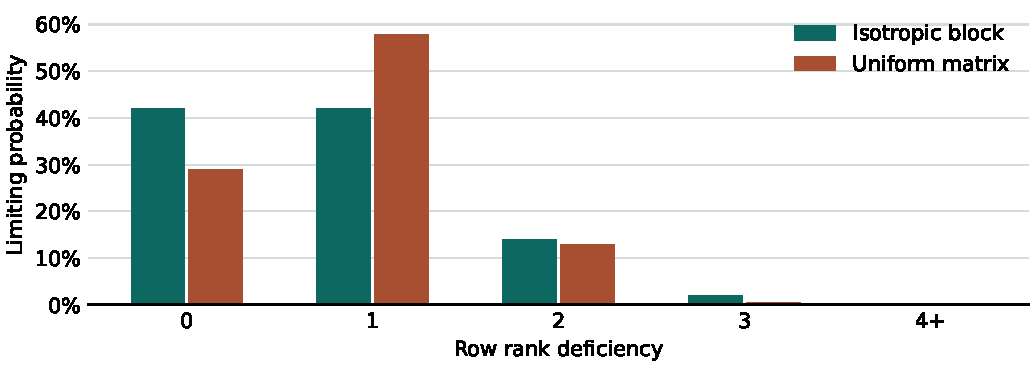
\includegraphics[width=.83\linewidth]{figures/rank_laws.pdf}
\caption{A square block over $\mathbb F_2$ with isotropic test spaces, as the ambient dimension tends to infinity. The probability of losing exactly one row of rank falls from $0.577576$ to $0.419422$. Its difference, $0.158154$, is the limiting total variation distance for the entire matrix.}
\end{figure}

The Lagrangian intersection count used when $c=0$ also appears in Richard Kueng and David Gross, \emph{Qubit stabilizer states are complex projective 3-designs}, Corollary~2 (\href{https://arxiv.org/abs/1510.02767}{arXiv:1510.02767}). The distribution comparison here concerns the full rectangular block and its distance from independent uniform entries. Ofir Gorodetsky's Theorem~1.8 in \emph{Statistics of entries of matrices from the general linear group over a finite field} treats random $\operatorname{GL}_n$ blocks (\href{https://arxiv.org/abs/2610.29305}{arXiv:2610.29305}). In that setting $n-\min(a,b)\to\infty$ suffices. Along the symplectic family just constructed this quantity grows without bound, yet the full-row-rank test detects a nonvanishing discrepancy. The symplectic result thus answers a counterpart of the finite-field block question. Its proof uses neither RH nor GRH. The boundary calculation quantifies the discrepancy at each fixed deficit in a uniform theorem. It leaves scope for finer estimates when the two specific subspaces are known.
